\begin{figure}[!htbp]
\centering
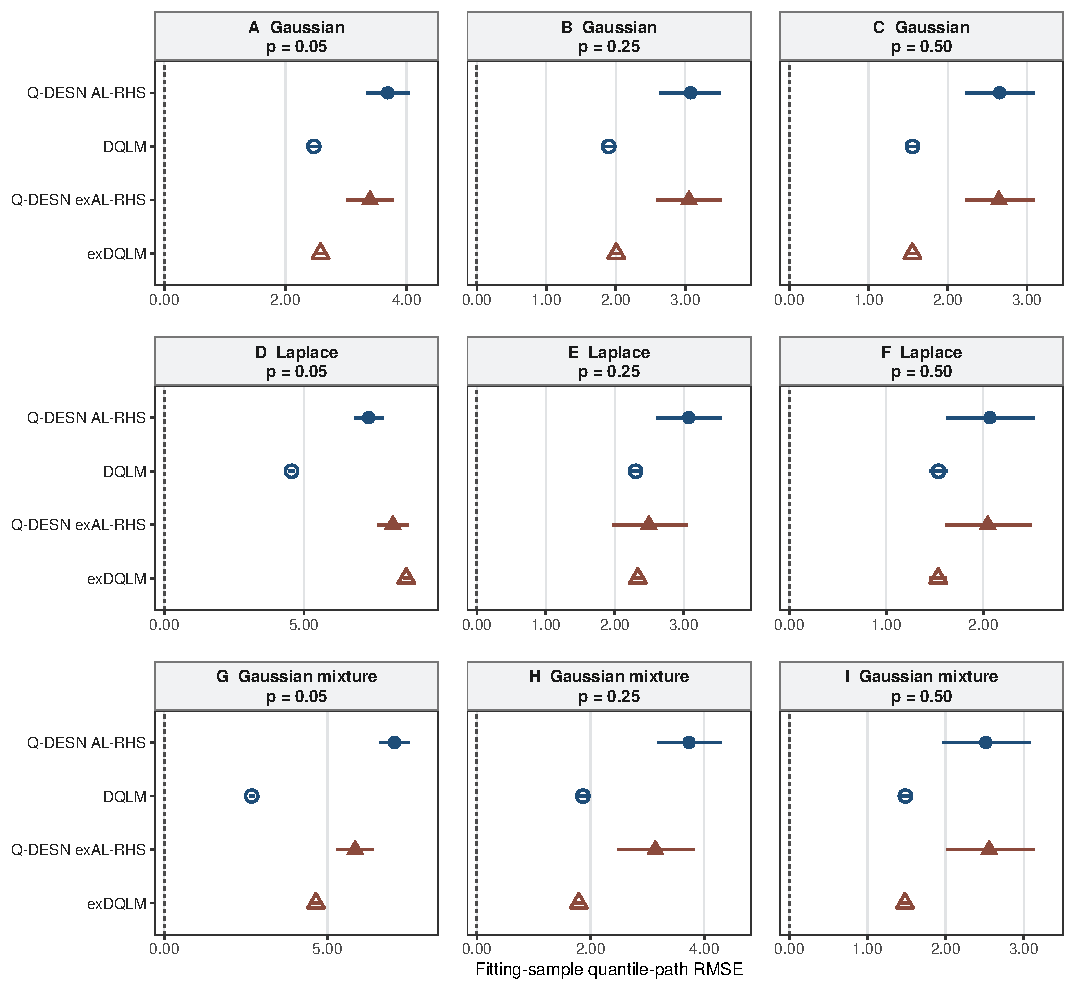
\includegraphics[width=0.98\textwidth]{figures/independent_simulation/qdesn_validation_500obs_v14_vb_fit_rmse_intervals.pdf}
\caption{Variational Bayes posterior uncertainty for fit RMSE in the single-quantile simulation study. Horizontal segments show equal-tailed approximate 95\% variational posterior intervals; crosses mark posterior means. Each panel uses its own horizontal scale, and lower values are better. The black dashed line marks the exact DGP oracle value of zero for this conditional-quantile path-error criterion. Intervals condition on the simulated data, evaluation design, and case-specific model specification.}
\label{fig:simulation-500obs-vb-fit-rmse-intervals}
\end{figure}

\begin{figure}[!htbp]
\centering
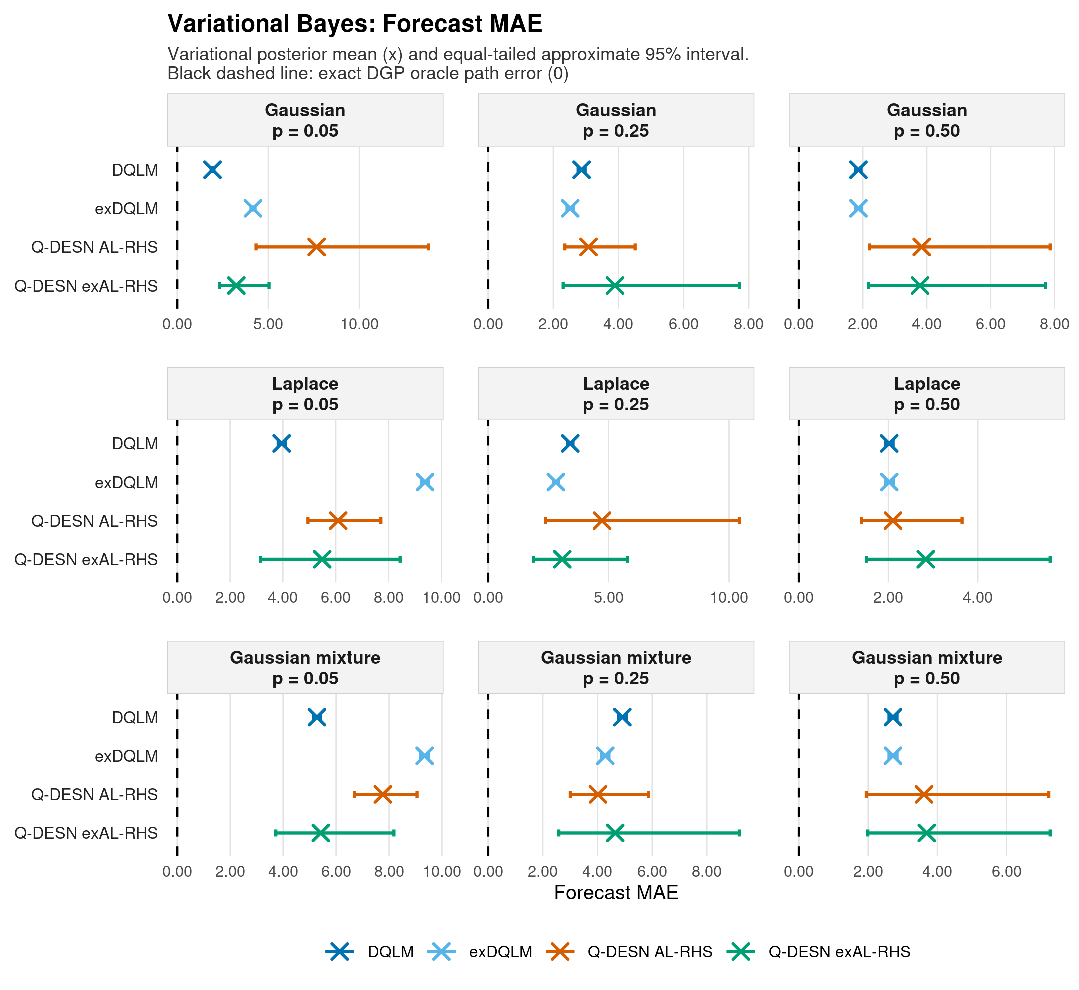
\includegraphics[width=0.98\textwidth]{figures/independent_simulation/qdesn_validation_500obs_v14_vb_forecast_mae_intervals.pdf}
\caption{Variational Bayes posterior uncertainty for forecast MAE in the single-quantile simulation study. Horizontal segments show equal-tailed approximate 95\% variational posterior intervals; crosses mark posterior means. Each panel uses its own horizontal scale, and lower values are better. The black dashed line marks the exact DGP oracle value of zero for this conditional-quantile path-error criterion. Intervals condition on the simulated data, evaluation design, and case-specific model specification.}
\label{fig:simulation-500obs-vb-forecast-mae-intervals}
\end{figure}

\begin{figure}[!htbp]
\centering
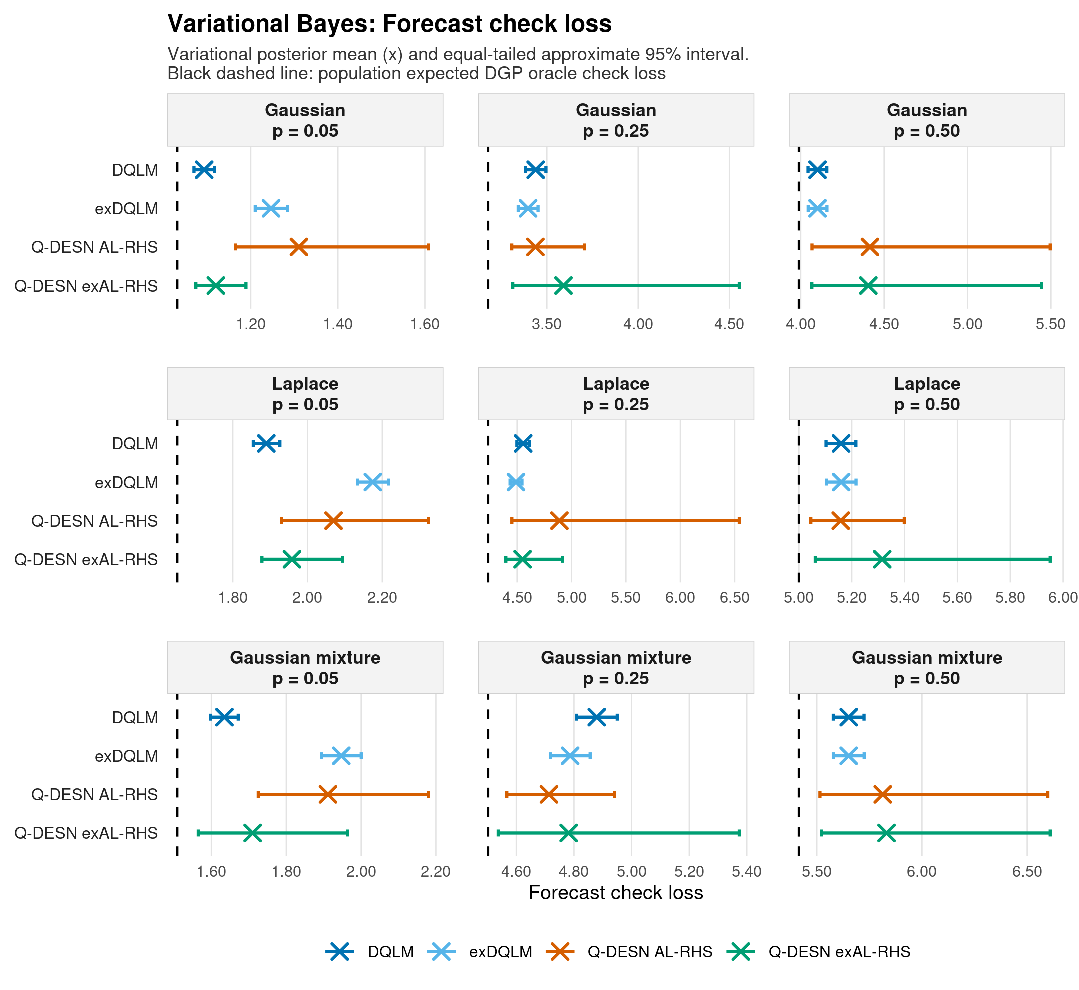
\includegraphics[width=0.98\textwidth]{figures/independent_simulation/qdesn_validation_500obs_v14_vb_forecast_check_loss_intervals.pdf}
\caption{Variational Bayes posterior uncertainty for forecast check loss in the single-quantile simulation study. Horizontal segments show equal-tailed approximate 95\% variational posterior intervals; crosses mark posterior means. Each panel uses its own horizontal scale, and lower values are better. The black dashed line marks the population expected check loss at the true conditional quantile. Because the intervals condition on one simulated series, finite-sample check-loss summaries may cross this population reference. Intervals condition on the simulated data, evaluation design, and case-specific model specification.}
\label{fig:simulation-500obs-vb-forecast-check-loss-intervals}
\end{figure}
